\documentclass[11pt,a4paper]{article}

\usepackage{geometry}
\geometry{margin=2.5cm}
\usepackage{setspace}
\usepackage{booktabs}
\usepackage{longtable}
\usepackage{hyperref}
\usepackage{graphicx}
\usepackage{tabularx}
\usepackage{booktabs}
\usepackage{float}
\usepackage{tikz}
\usepackage{blindtext}
\usepackage{hyperref}
\usetikzlibrary{arrows.meta, positioning}
\usepackage{comment}

\hypersetup{
    colorlinks=true,
    linkcolor=blue,
    filecolor=magenta,      
    urlcolor=cyan,
    pdftitle={Overleaf Example},
    pdfpagemode=FullScreen,
    }
\renewcommand{\thesection}{\arabic{section}}

\onehalfspacing

\title{\textbf{SOCRATES: Guidelines for data formatting}}
% \large Social Contact Survey Data}
% \author{SOCRATES Maintainers}
\date{}

\begin{document}
\maketitle \vspace{-1.2cm}

\section{Introduction and scope}
\noindent
The web repository \href{https://socialcontactdata.org}{socialcontactdata.org} curates and disseminates data from social contact surveys conducted worldwide.
By providing a common framework for data organisation and documentation, the repository aims to facilitate data sharing, comparability across studies, and reuse in modelling and public health research. Datasets hosted on the repository are intended for use with the \href{https://lwillem.shinyapps.io/socrates_rshiny/}{SOCRATES tools} and the \href{https://cran.r-project.org/web/packages/socialmixr/index.html}{socialmixr} R package, both of which rely on standardised data structures and variable definitions to enable consistent data access, validation, and downstream analysis. To support these goals, contributed datasets are required to follow a set of general formatting rules. 

\section{Identifiers and naming conventions}
\subsection{Study identifier (NAMETAG)}
Each social contact survey included in the repository is assigned a unique \texttt{NAMETAG} for identification purposes. The \texttt{NAMETAG} has the following structure:
\[
\texttt{NAMETAG} = \texttt{NAME\_YEAR\_COUNTRY}
\]
where \texttt{NAME} corresponds to the surname of the first author of the earliest publication presenting the dataset, \texttt{YEAR} to the year of that publication, and \texttt{COUNTRY} to the English name of the country in which the survey data were collected. If data were collected in multiple countries, the dataset must be split by country and assigned one \texttt{NAMETAG} per country.

\medskip
\noindent\textbf{Example:}
For a social contact survey conducted in Belgium and published by Doe et al.\ in 2012, the corresponding \texttt{NAMETAG} is:
\[
\texttt{DOE\_2012\_BELGIUM}.
\]
All data files must be provided as plain text comma-separated values (\texttt{.csv}) files, using a comma (\texttt{,}) as field delimiter and must not contain row names or implicit index columns. 

\subsection{Record and entity identifiers}
The standardised social contact data data structure (as utilized by \href{https://cran.r-project.org/web/packages/socialmixr/index.html}{socialmixr} and the \href{https://lwillem.shinyapps.io/socrates_rshiny/}{SOCRATES tools}) relies on a set of identifiers that operate at different levels of the data.
Each identifier has a unique and well-defined role and must be used consistently across files. \textbf{In this standardised format, these identifiers are implemented as column names and are used to link records across data tables.}

\begin{itemize}
    \item \texttt{part\_id}: identifies a single unique identifier for the respondent's entry. This ID must be unique across the entire submission.
    \item \texttt{sday\_id}: identifies the calendar date associated with a given \texttt{part\_id}, in \texttt{YYYYMMDD} format.
    \item \texttt{cont\_id}: identifies a single contact event.
    \item \texttt{hh\_id}: identifies a household.
    \item \texttt{panel\_id}: identifies the same underlying individual across multiple survey rounds or waves (optional).
\end{itemize}

\noindent \textbf{Note:} all variable names defined in this guideline are case-sensitive and must match their definitions exactly. For example, \texttt{part\_id} must not be renamed to \texttt{Part\_ID}, \texttt{participant\_id}, or \texttt{partID}. Deviations will prevent correct parsing by the \href{https://lwillem.shinyapps.io/socrates_rshiny/}{SOCRATES} and \href{https://cran.r-project.org/web/packages/socialmixr/vignettes/socialmixr.html}{socialmixr} compatible tools.

\subsection{Missing values}
All missing or not-collected values should be encoded as \texttt{NA}. Empty cells, whitespace, placeholder values (e.g.\ \texttt{-99}, \texttt{999}), or empty strings are not recommended. The missing value encoding should be used consistently across all files and variables, regardless of data type.

\section{General formatting rules}
\noindent Each survey should be organised as a set of relational datasets, with one file per data entity. To ensure consistency across submissions, the following files are required:

\begin{table}[h]
\centering
% \caption{Required data files and relational structure}
\label{tab:datafiles}
\resizebox{\textwidth}{!}{
    \begin{tabular}{llll}
    \toprule
    \textbf{File} & \textbf{Description} &
    \textbf{Primary key}\footnotemark[1] &
    \textbf{Foreign key(s)}\footnotemark[2] \\
    \midrule
    Participant file &
    Participant-level information &
    \texttt{part\_id} &
    \texttt{hh\_id} \\
    
    Contact file &
    Contact-level social interactions &
    \texttt{contact\_id} &
    \texttt{sday\_id}, \texttt{part\_id} \\
    
    Household file &
    Household-level information &
    \texttt{hh\_id} &
    -- \\
    
    Survey day file &
    Survey day characteristics &
    \texttt{sday\_id} &
    \texttt{part\_id} \\
    
    Time-use file (optional) &
    Time-use information per survey day &
    \texttt{part\_id} &
    \texttt{sday\_id} \\
    
    Dictionary file &
    Variable definitions and coding &
    -- &
    -- \\
    \bottomrule
    \end{tabular}
    }
\end{table}
\footnotetext[1]{A primary key uniquely identifies records within a dataset.}
\footnotetext[2]{A foreign key references a primary key in another dataset to enable linkage across files.}

\noindent Participant-, contact-, and household-level information must each be provided in two separate files. For each data entity, contributors should distinguish between:

\begin{itemize}
    \item a \textbf{common file}, containing variables that are typically available across most social contact surveys and are required for integration into the \textbf{socialmixr R package} and the \textbf{SOCRATES platform};
    \item an \textbf{extra file}, containing survey-specific variables that are not part of the common data structure. 
\end{itemize}
\noindent The common files are used for harmonisation and standard analyses, whereas the extra files preserve additional information specific to the original survey. 
The \textbf{common} and \textbf{extra} files for a given data entity can be merged using the primary key. 
The extra file must contain only variables that are not included in the corresponding common file; variables defined in the common file must not be duplicated. 
The name of each file must start with the corresponding \texttt{NAMETAG}.

\section{File specifications} 
\label{sec:file_spesifications}
\noindent The sections below specify the required variables for each \textbf{common} data file, grouped by data entity. All variables listed for a \textbf{common} file must be present as columns in the corresponding dataset. If a variable was not collected in a given survey, the column must still be included and filled with \texttt{NA} values. Only the \textbf{common} files are subject to this requirement (the structure of the common file must not be modified); extra files may contain an arbitrary set of additional variables. 

\begin{comment}
\begin{figure}[h]
\centering
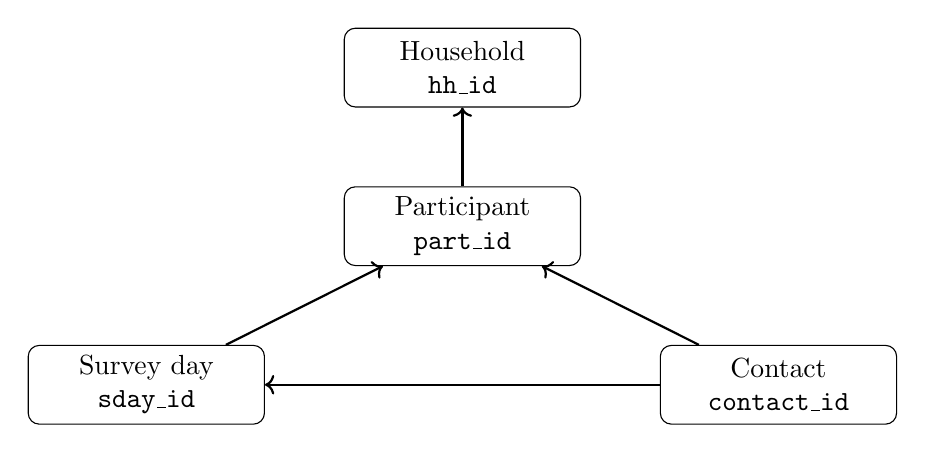
\begin{tikzpicture}[
  entity/.style={draw, rectangle, rounded corners, align=center, minimum width=3cm, minimum height=1cm},
  arrow/.style={->, thick}
]

\node[entity] (hh) {Household\\\texttt{hh\_id}};
\node[entity, below=of hh] (part) {Participant\\\texttt{part\_id}};
\node[entity, below left=of part] (sday) {Survey day\\\texttt{sday\_id}};
\node[entity, below right=of part] (contact) {Contact\\\texttt{contact\_id}};

\draw[arrow] (part) -- (hh);
\draw[arrow] (sday) -- (part);
\draw[arrow] (contact) -- (part);
\draw[arrow] (contact) -- (sday);

\end{tikzpicture}
\caption{Relational structure of SOCRATES data files}
\label{fig:relational_structure}
\end{figure}
\end{comment}

\begin{enumerate}
    \item \textbf{Participant common file} (file name: \texttt{NAMETAG\_participant\_common.csv}) \\
    The participant common file contains core demographic information for each survey participant, with exactly one record provided per participant. Longitudinal linkage across survey rounds is handled via \texttt{panel\_id} (see Section~\ref{sec:longitudinal}).

    \begin{table}[H]
    \centering
    % \caption{Participant common file schema}
    \label{tab:participant_common}
    \begin{tabularx}{\textwidth}{l l l X}
    \toprule
    \textbf{Column} & \textbf{Type} & \textbf{Coding} & \textbf{Notes} \\
    \midrule
    \texttt{part\_id} & string / integer & unique identifier & Primary key; unique within the submission. \\
    \texttt{hh\_id} & string / integer & household identifier & Foreign key to the household common file; use \texttt{NA} if not collected. \\
    \texttt{part\_age} &  integer & years &
    Exact age in years (numeric). Use \texttt{NA} if not collected. \\
    \texttt{part\_age\_est\_min} &
    integer &
    years &
    Lower bound of estimated age interval (numeric); otherwise \texttt{NA}. \\

    \texttt{part\_age\_est\_max} &
    integer &
    years &
    Upper bound of estimated age interval (numeric); otherwise \texttt{NA}. \\

    \texttt{part\_gender} & string & \texttt{F}, \texttt{M}, \texttt{O} & \texttt{O} denotes a non-binary or other gender category as defined by the original survey; use \texttt{NA} if not collected. \\
    \bottomrule
    \end{tabularx}
    \end{table}

    \noindent\textbf{Age encoding rules:} \\
    Participant age must be provided using one of the following approaches:
    \begin{itemize}
        \item     If exact age in completed years is known, it should be recorded in \texttt{part\_age} and both \texttt{part\_age\_est\_min} and \texttt{part\_age\_est\_max} must be set to \texttt{NA}.
        \item If age is reported as a range or estimated interval, the lower and upper bounds must be recorded in \texttt{part\_age\_est\_min} and \texttt{part\_age\_est\_max}, respectively, and \texttt{part\_age} must be set to \texttt{NA}.
    \end{itemize}
    Providing age information redundantly across these fields is not recommended.
    
    \item \textbf{Contacts common file} (file name: \texttt{NAMETAG\_contact\_common.csv})\\
    The contacts common file contains contact-level information. Each record corresponds to one contact reported by one participant on one survey day. Multiple location indicators may be TRUE for a single contact if applicable. If studies collect additional or alternative location categories beyond those defined in the common file, these must be stored in the contacts extra file. The information to be included and the required order are the following:
        
    \begin{table}[H]
    \centering
    \resizebox{0.95\textwidth}{!}{
    \begin{tabularx}{\textwidth}{l l l X}
    \toprule
    \textbf{Column} & \textbf{Type} & \textbf{Coding} & \textbf{Notes} \\
    \midrule
    \texttt{part\_id} &
    string / integer &
    participant identifier &
    Foreign key to the participant file (\texttt{part\_id}). \\
    

    \texttt{cnt\_id} &
    string / integer &
    unique identifier &
    Primary key. Must be unique within the survey submission. \\
    
    \texttt{cnt\_gender} &
    string &
    \texttt{F}, \texttt{M}, \texttt{O} &
    Gender of the contacted person; use \texttt{NA} if not collected. \\
    
    \texttt{cnt\_age\_exact} &
    integer &
    years &
    Exact age of the contacted person; otherwise \texttt{NA}. \\
    
    \texttt{cnt\_age\_est\_min} &
    integer &
    years &
    Lower bound of estimated age interval; otherwise \texttt{NA}. \\
    
    \texttt{cnt\_age\_est\_max} &
    integer &
    years &
    Upper bound of estimated age interval; otherwise \texttt{NA}. \\
    
    \texttt{cnt\_age\_multi} &
    string / integer &
    category code &
    Age-class code if reported in categories$^{*}$\\
    
    \texttt{cnt\_home} &
    boolean &
    \texttt{TRUE/FALSE} &
    Contact occurred at the participant's home; use \texttt{NA} if not collected.\\

    \texttt{cnt\_work} &
    boolean &
    \texttt{TRUE/FALSE} &
    Contact occurred at the participant's workplace; use \texttt{NA} if not collected.\\

    \texttt{cnt\_school} &
    boolean &
    \texttt{TRUE/FALSE} &
    Contact occurred at school; use \texttt{NA} if not collected.\\

    \texttt{cnt\_transport} &
    boolean &
    \texttt{TRUE/FALSE} &
    Contact occurred while using transport; use \texttt{NA} if not collected.\\

    \texttt{cnt\_leisure} &
    boolean &
    \texttt{TRUE/FALSE} &
    Contact occurred during a leisure activity; use \texttt{NA} if not collected.\\

    \texttt{cnt\_others} &
    boolean &
    \texttt{TRUE/FALSE} &
    Contact occurred at any other location; use \texttt{NA} if not collected.\\
    
    \texttt{frequency\_multi} &
    string / integer &
    category code &
    Frequency code if multiple frequency options are used$^{*}$.\\
    
    \texttt{duration\_exact} &
    numeric &
    minutes (or specify) &
    Exact duration if reported numerically; otherwise \texttt{NA}. \\
    
    \texttt{duration\_multi} &
    string / integer &
    category code &
    Duration-class code if reported in categories$^{*}$. \\
    
    \texttt{phys\_contact} &
    boolean &
    \texttt{TRUE/FALSE} &
    Indicator for physical contact; use \texttt{NA} if not collected. \\
    
    \bottomrule
    \end{tabularx}
    }
    \end{table}
    
    \noindent
    ($^{*}$) If categorical codes are used, the dictionary file must include the complete mapping from codes to labels.

    \item \textbf{Household common file} (file name: \texttt{NAMETAG\_hh\_common.csv}) \\
    The household common file contains core household-level information. Exactly one record must be provided per household.

    \begin{table}[H]
        \centering
%        \caption{Household common file schema}
%        \label{tab:household_common}
        \begin{tabularx}{\textwidth}{l l l X}
        \toprule
        \textbf{Column} & \textbf{Type} & \textbf{Coding} & \textbf{Notes} \\
        \midrule
        \texttt{hh\_id} &
        string / integer &
        unique identifier &
        Primary key. Must be unique within the survey submission. \\
        
        \texttt{country} &
        string &
        ISO alpha-2 code &
        Country in which the survey data were collected, encoded using ISO 3166-1 alpha-2 (e.g.\ \texttt{BE} for Belgium, and \texttt{FR} for France). \\

        \texttt{hh\_size} &
        integer &
        count &
        Household size; use \texttt{NA} if not collected. \\
        
        \bottomrule
        \end{tabularx}
    \end{table}

    \item \textbf{Survey day file} (file name: \texttt{NAMETAG\_sday.csv})\\
    The survey day file contains metadata describing the calendar date associated with each \texttt{part\_id}. 

    \begin{table}[H]
    \centering
%    \caption{Survey day common file schema}
%    \label{tab:sday_common}
    \begin{tabularx}{\textwidth}{l l l X}
    \toprule
    \textbf{Column} & \textbf{Type} & \textbf{Coding} & \textbf{Notes} \\
    \midrule
    \texttt{part\_id} &
    string / integer &
    participant identifier &
    Primary key to the participant file (\texttt{part\_id}). \\

    \texttt{sday\_id} &
    string &
    \texttt{YYYYMMDD} &
    Foreign key. Survey date identifier. \\
    
    \texttt{day} &
    integer &
    1--31 &
    Calendar day corresponding to \texttt{sday\_id}. \\
    
    \texttt{month} &
    integer &
    1--12 &
    Calendar month corresponding to \texttt{sday\_id}. \\
    
    \texttt{year} &
    integer &
    4-digit year &
    Calendar year corresponding to \texttt{sday\_id}. \\
    
    \texttt{dayofweek} &
    integer &
    0--6 &
    Day of week (0=Sunday, 1=Monday, \ldots, 6=Saturday). \\
    
    \bottomrule
    \end{tabularx}
    \end{table}
    
    \item \textbf{Dictionary file} (file name: \texttt{NAMETAG\_dictionary.xlsx})

    The dictionary file documents all variables included in the submitted datasets. It must include, for each variable:
    \begin{enumerate}
        \item  the variable name
        \item a short description
        \item the data type (e.g.\ integer, floating point, string)
        \item the allowed values and their meaning (for categorical variables).
    \end{enumerate}
    
    \noindent The dictionary must be organised by file.
    If a spreadsheet format is used (e.g.\ \texttt{.xlsx}), it should contain one sheet per data file.

    \item \textbf{Extra files} (file name: \texttt{NAMETAG\_xxx\_extra.csv}) \\
    The \textbf{extra} files contain survey-specific variables that are not included in the corresponding \textbf{common} file. For each data entity, the common and extra files must share the same primary key, which ensures a one-to-one match between records across data tables.
\end{enumerate}

\noindent \textbf{Commonly missed step: mandatory empty columns} \\
All variables listed in Section~\ref{sec:file_spesifications} must be present as columns, even if no data were collected. In such cases, columns must be included and filled with NA. Deleting unused columns will break compatibility with the socialmixr import standard.

\section{Longitudinal and panel studies}
\label{sec:longitudinal}
   In longitudinal or panel studies, participants may be observed on multiple survey occasions; in such cases, time-varying information must be represented using separate \texttt{part\_id} values, linked via \texttt{panel\_id} where applicable. Specifically,
\begin{itemize}
    \item \texttt{part\_id} must uniquely identify each participant--survey instance (i.e.\ each record) and must remain unique across the entire submission.
    \item \texttt{panel\_id} should be used to identify the same underlying individual across multiple survey rounds or waves.
\end{itemize}

\noindent
Records corresponding to the same individual across different survey rounds must share the same \texttt{panel\_id} but have distinct \texttt{part\_id} values. 
The \texttt{panel\_id} is not included in the participant common file and, when available, must be provided in the participant extra file and linked using \texttt{part\_id}.

\begin{figure}[H]
\centering
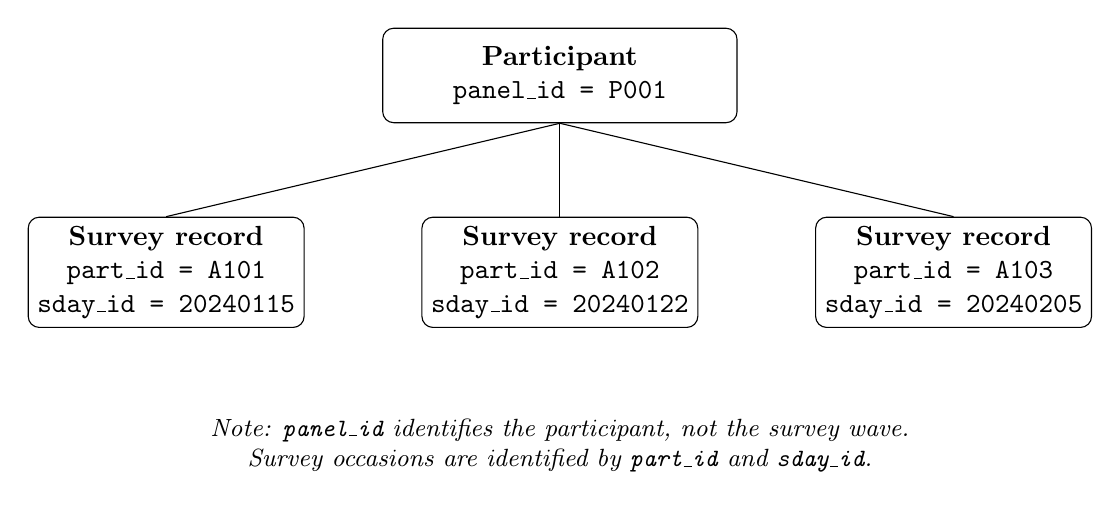
\begin{tikzpicture}[
    box/.style={draw, rectangle, rounded corners, align=center, minimum width=3.5cm, minimum height=1.4cm},
    pid/.style={draw, rectangle, rounded corners, align=center, minimum width=4.5cm, minimum height=1.2cm},
    line/.style={-}
]

% Panel ID (underlying individual)
\node[pid] (panel) at (0,2.5) {\textbf{Participant}\\ \texttt{panel\_id = P001}};

% Survey occasions
\node[box] (occ1) at (-5,0) {\textbf{Survey record}\\
\texttt{part\_id = A101}\\
\texttt{sday\_id = 20240115}};

\node[box] (occ2) at (0,0) {\textbf{Survey record}\\
\texttt{part\_id = A102}\\
\texttt{sday\_id = 20240122}};

\node[box] (occ3) at (5,0) {\textbf{Survey record}\\
\texttt{part\_id = A103}\\
\texttt{sday\_id = 20240205}};

% Connections
\draw[line] (panel.south) -- (occ1.north);
\draw[line] (panel.south) -- (occ2.north);
\draw[line] (panel.south) -- (occ3.north);

% Optional note
\node[align=center, font=\small] at (0,-2.2)
{\textit{Note: \texttt{panel\_id} identifies the participant, not the survey wave.}\\
\textit{Survey occasions are identified by \texttt{part\_id} and \texttt{sday\_id}.}};

\end{tikzpicture}
\caption{Schematic representation of participant identifiers in longitudinal studies.}
\end{figure}

\section{Zenodo submission and metadata requirements}

SOCRATES-formatted datasets are disseminated via \href{https://zenodo.org}{Zenodo} to support long-term archiving, versioning, and reuse. 
To ensure datasets hosted on \href{https://socialcontactdata.org}{socialcontactdata.org} are discoverable and interoperable, contributors must adhere to the following Zenodo metadata requirements. \\ 

\noindent \textbf{Versioning} \\
Each dataset release must specify a clear version number using a numeric scheme (e.g.\ \texttt{v1.0}, \texttt{v1.1}). 
New versions must be created for any change affecting data content, structure, or documentation. \\

\noindent \textbf{Community and keywords} \\
All submissions must be associated with the \textit{Social Contact Data} Zenodo community.
Contributors are encouraged to include keywords such as \texttt{social contacts}, \texttt{contact data}, and \texttt{contact matrix} to facilitate discovery. \\

\noindent Note that each dataset corresponds to a single survey implementation. If multiple surveys are conducted within the same country and year, they must be submitted as separate datasets, each with its own Zenodo record and unique identifier. The information provided in the Zenodo (title, description, dates, and geographic scope) must be consistent with the contents of the submitted data files. 

\section{Submission workflow}

To make a dataset available through \href{https://socialcontactdata.org}{socialcontactdata.org}, contributors must complete the following steps:
\begin{enumerate}
    \item Format the dataset according to the SOCRATES data formatting guidelines described in this document.
    \item Upload the formatted dataset and accompanying documentation to \href{https://zenodo.org}{Zenodo}.
    \item Contact the \href{https://socialcontactdata.org}{socialcontactdata.org} team to request that the Zenodo record be linked and indexed on the platform.
\end{enumerate}


\section{Contact and support}
Questions regarding data formatting or submission should be directed to:
\begin{center}
\texttt{[socialcontactdata@gmail.com]}
\end{center}

\end{document}
